% This is the overview document of the RTPC

The CLAS12 Radial Time Projection Chamber (RTPC)  is a cylindrical gaseous detector of radius 8 cm used in the BONuS12 experiment. This detector is made up of three layers of 40 cm long concentric GEM (Gaseous Electron Multiplier) cylinders as shown in figure \ref{fig:RTPC} and \ref{fig:bonus12}. The detector has two separate cylindrical volume: buffer volume extending from target wall (at radius r=3 mm from beamline) to the ground foil of the detector (at r =20 mm), and active volume extending from ground foil to the padboard at r = 80mm. Helium gas is used in the buffer, and mixture of He (80\%) and CO2 (20\%) is used in the active space. The gas system for the BONuS12 experiment is shown in figure \ref{fig:gas_system}.

\begin{figure}[H]
	\centering
	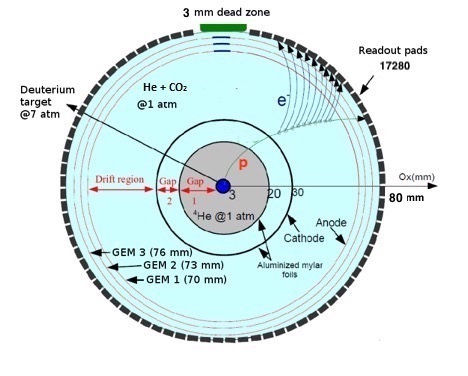
\includegraphics[scale=0.8]{rtpc}
	%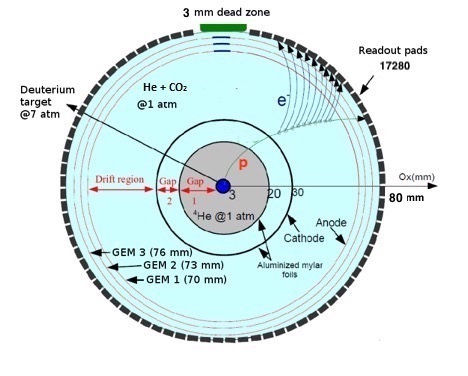
\includegraphics[width=11cm, height=9cm]{rtpc}
	\caption{Schematics of cross-section of BONuS12 RTPC and a proton track}
	\label{fig:RTPC}
\end{figure}

There are 7 high voltage channels to power up RTPC up to 7000V, but the current limit for the HV is extremely low. One high voltage channel is used for the cathode foil and the 6 others are connected to the GEMs. The end caps are powered via the inner most GEM foil and the cathode.

\begin{figure}[H]
	\centering
	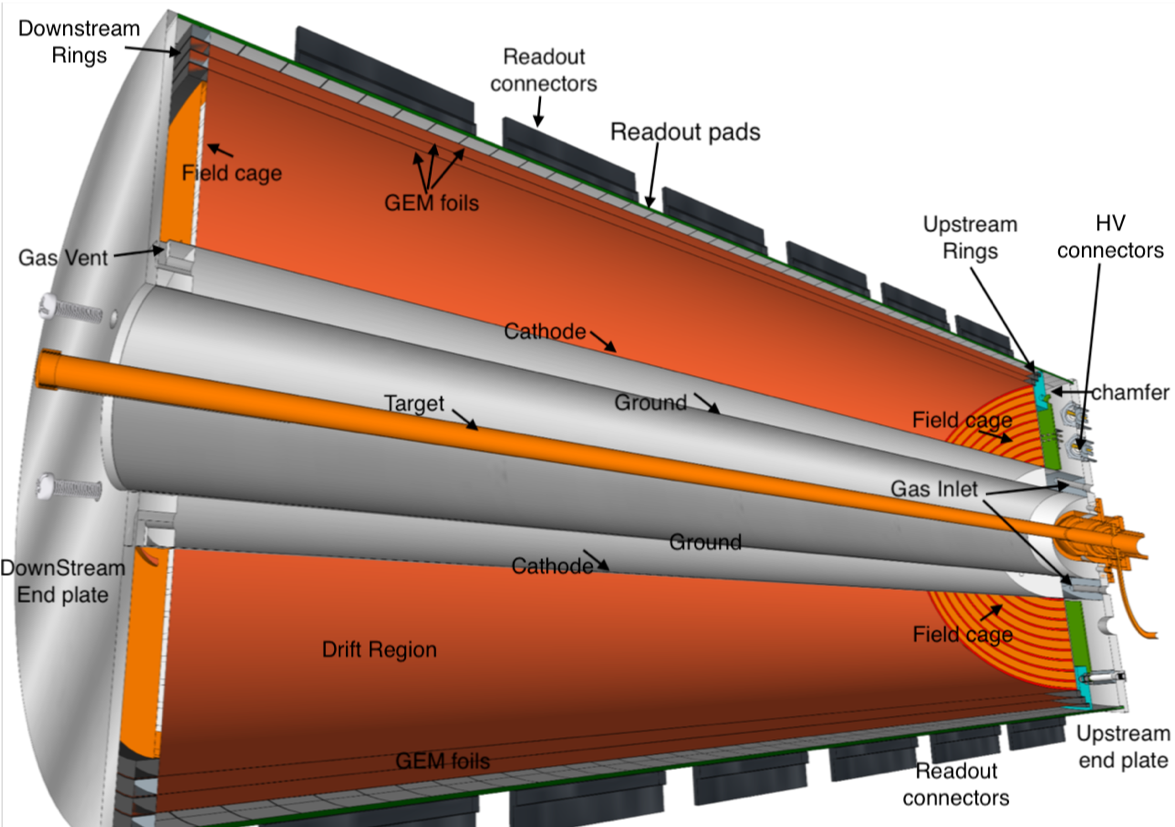
\includegraphics[height=7cm,width=12cm]{Bonus12}
	\caption{Longitudinal cross-sectional of BONuS12 RTPC}
	\label{fig:bonus12}
\end{figure}

When a proton traverses through the gas in the drift region of RTPC, atoms along its path are ionized which liberate electrons as shown in figure \ref{fig:RTPC}. An electric field maintained in the drift region drives these electrons toward GEMs. Avalanche occurs when electron passes through GEM because of the high electric field established between the two sides of each GEM. Three GEM foils are utilized to produce a large number of electrons which are collected from the readout board at the outer layer. The RTPC readout board comprises of a pattern of 4 mm$\crossproduct$2.75 mm conductive pads around the cylindrical detector. Electric signals obtained out of the readout board are used to project the position of the proton at particular time. In order to reconstruct a complete track of proton, we have 17280 readout pads around the RTPC and the DREAM based DAQ system is used to collect the signals from the pads.

\begin{figure}[H]
	\centering
	%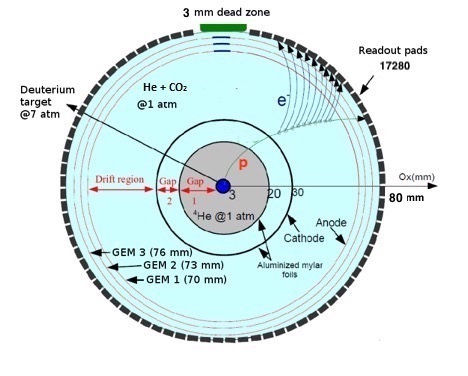
\includegraphics[scale=0.8]{rtpc}
	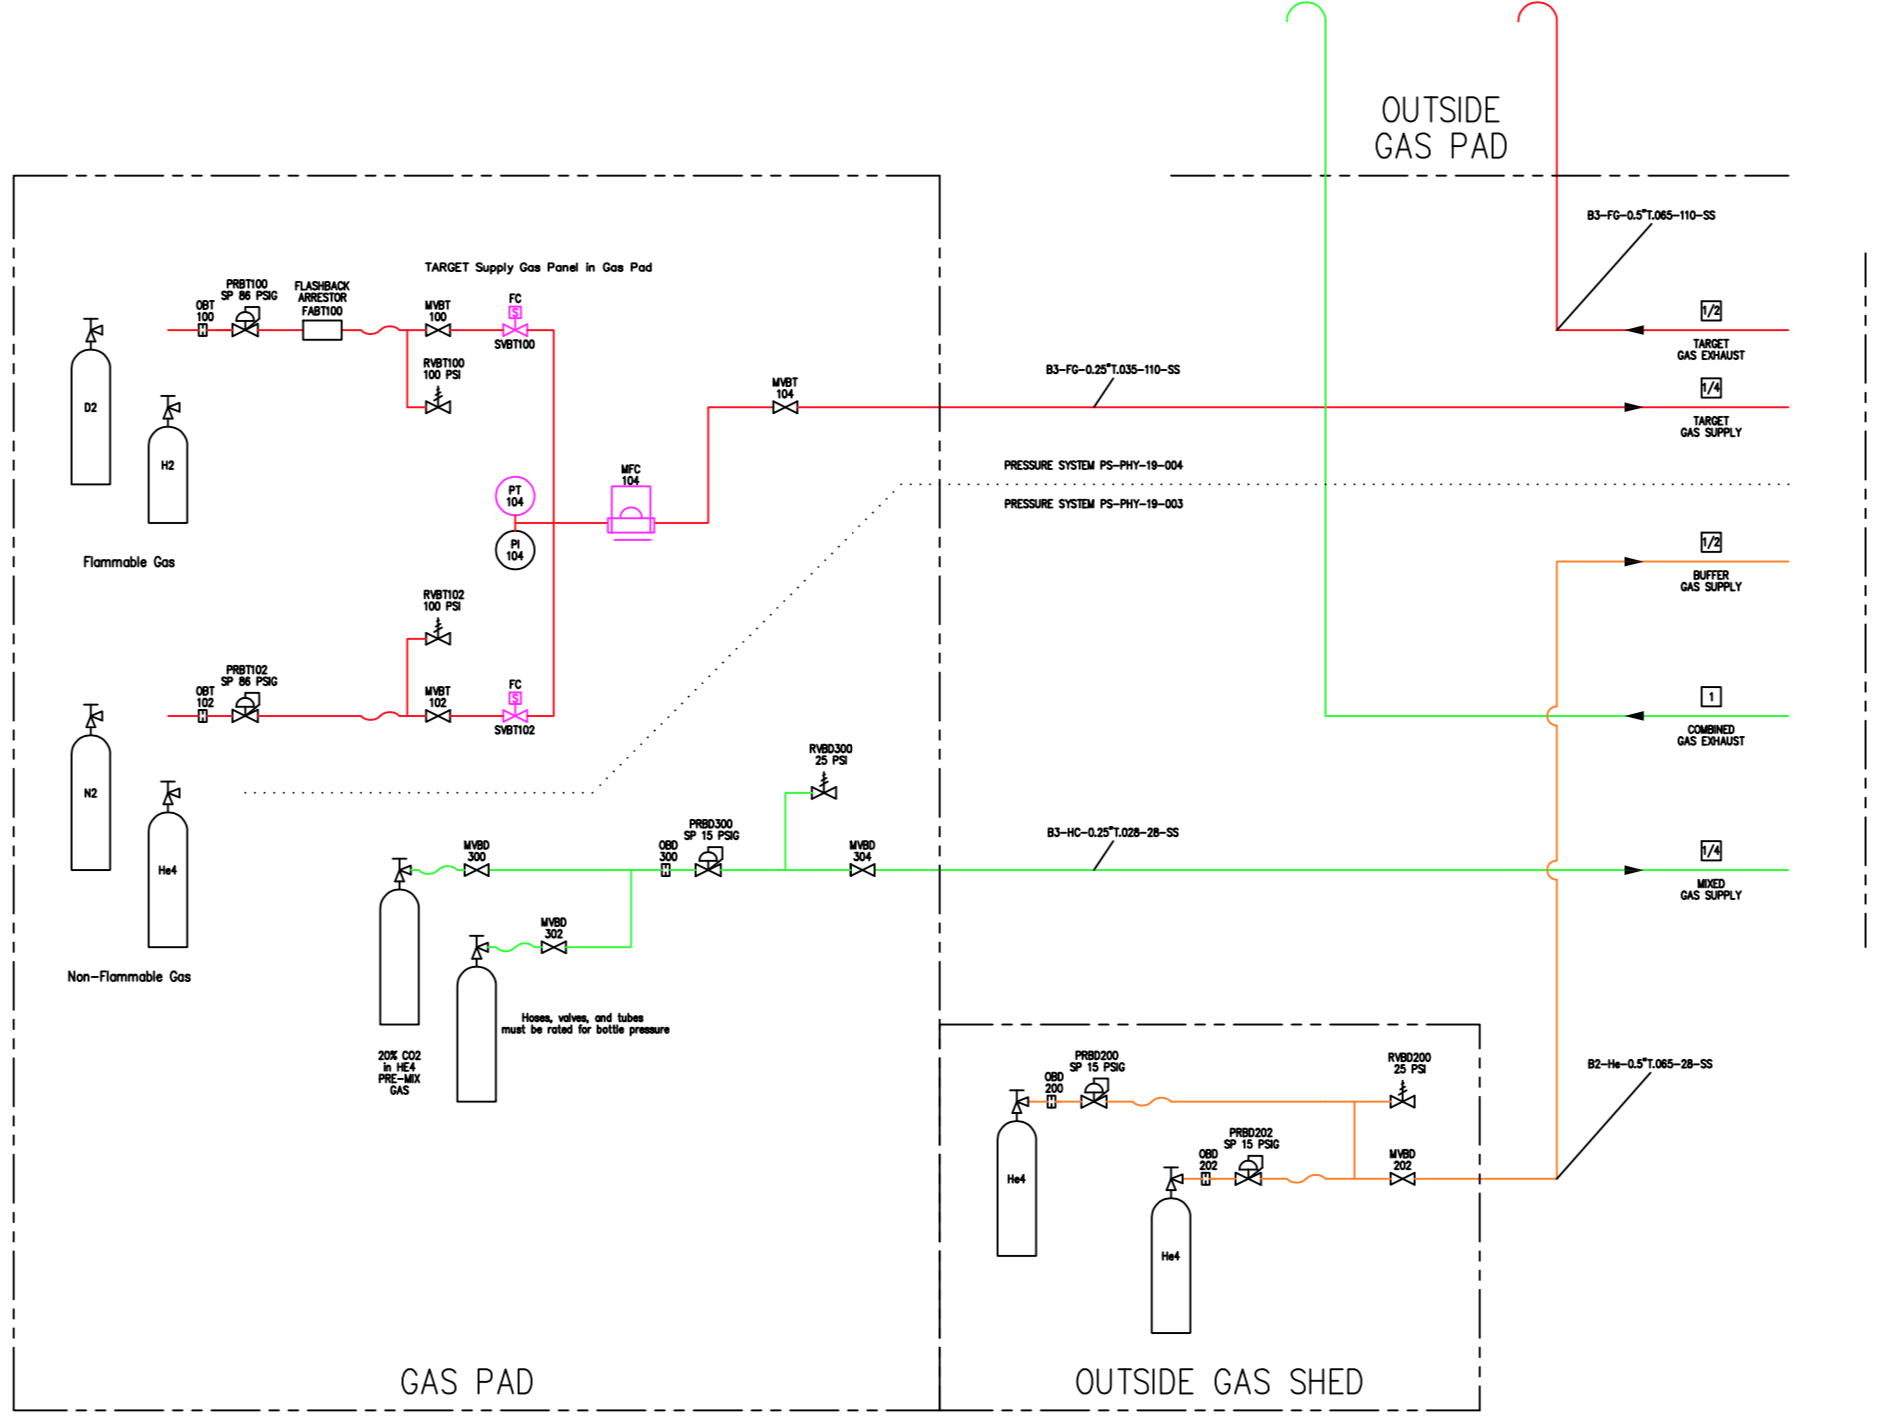
\includegraphics[width=5.5cm, height=6cm]{gas_shed}
	%\quad
	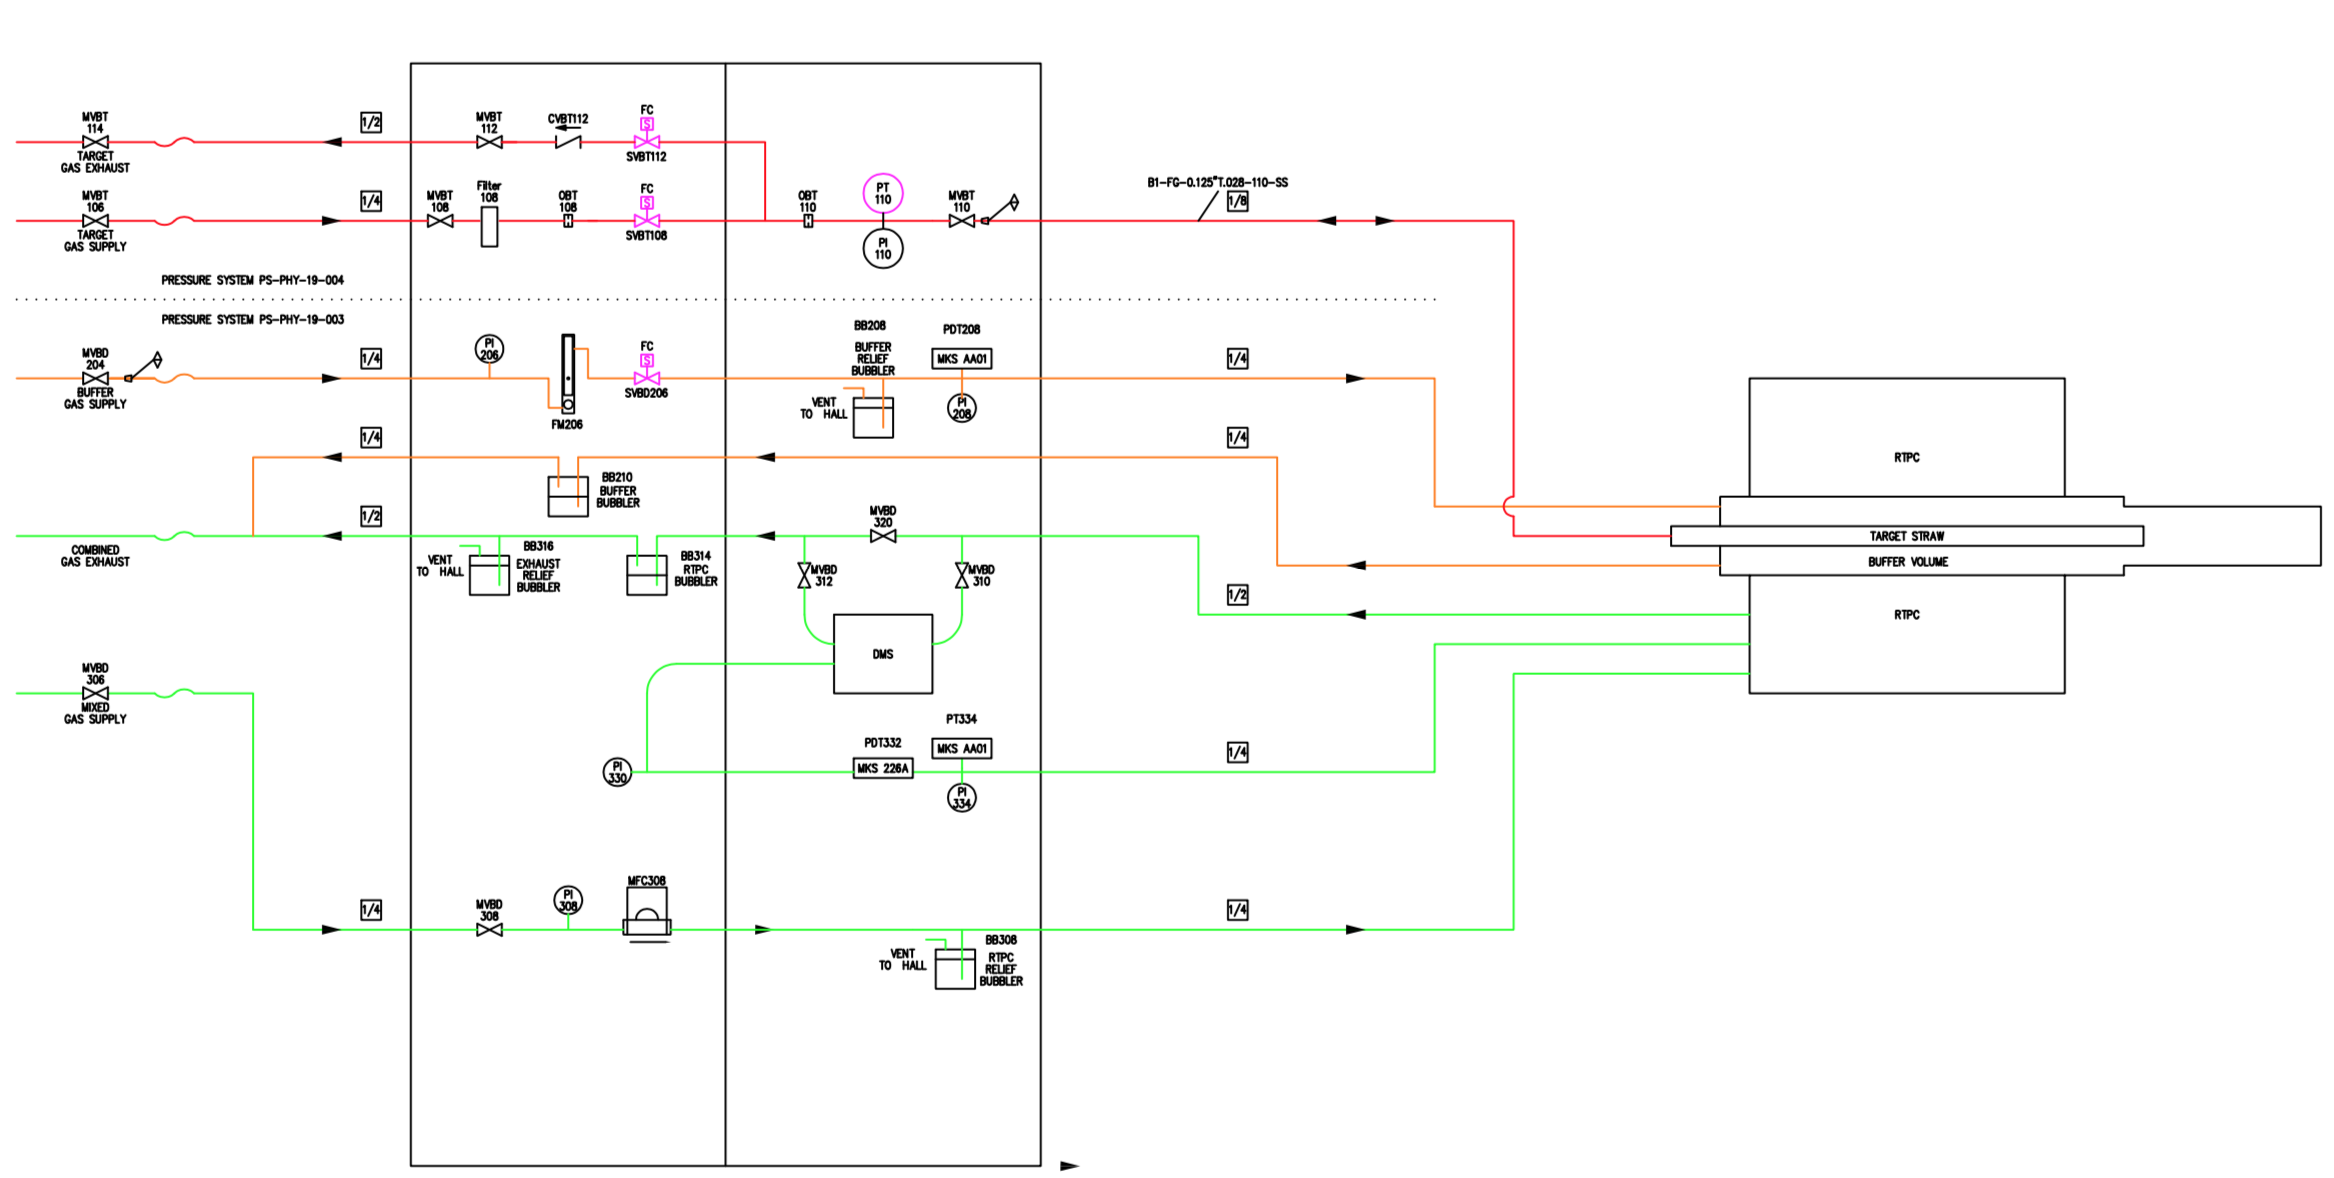
\includegraphics[width=8cm, height=5.3cm]{gas_flow}
	\caption{BONuS12 Gas System}
	\label{fig:gas_system}
\end{figure}

The DAQ system of RTPC consists of DREAM (Dead-timeless Readout Electronics Asic for Micromegas) chips developed by SACLAY group, primarily for the Micromegas detector of Hall B at Jefferson Lab. We replace the Micromegas detector by the RTPC detector in BONuS12, but would like to use the compact ASIC, DREAM. Each DREAM chip has 64 channels and each channel has integrated amplifier, filter, shaper, discriminator, and 512 cell analog circular buffer. So, signal from 64 readout pads are easily processed by a DREAM which are also sampled and temporarily stored in its buffer. Eight such chips are hosted by a FEU (Front End Unit), which is also supplemented by Flash-ADCs so as to get digitized data out from the FEU. Data are transferred from FEU to backend-unit using optical links as shown in figure \ref{fig:feu}. Zero suppression and Pedestal subtraction are implemented in FEUs for the BONuS12 experiment.

\begin{figure}[H]
	\centering
	\includegraphics[scale=1.3]{feu}
	%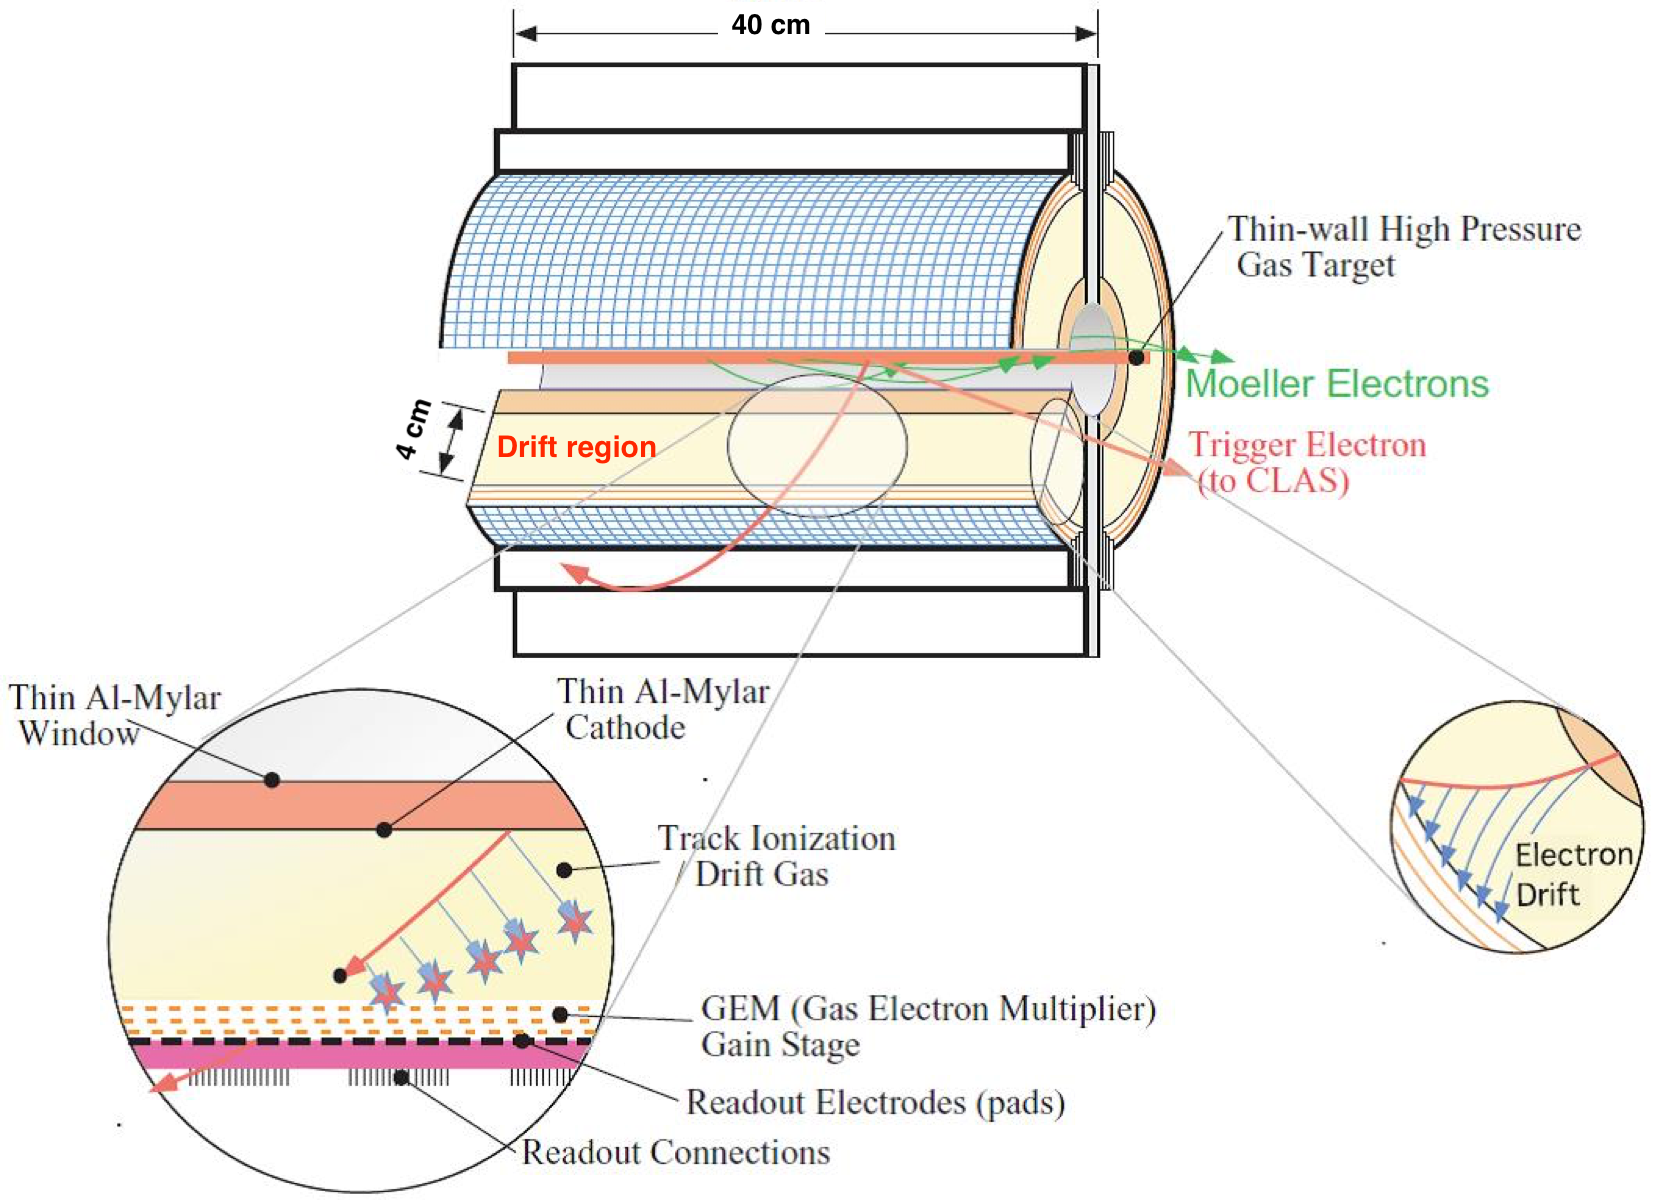
\includegraphics[width=5.4in, height=3.2in]{RTPC12}
	\caption{Schematics of Data Acquisition Electronics for the RTPC}
	\label{fig:feu}
\end{figure}